\documentclass{article}
\usepackage{amsmath}
\usepackage{amsfonts}
\usepackage[inline]{enumitem}
\usepackage[a4paper,margin=1in]{geometry}
\usepackage[normalem]{ulem}
\usepackage{graphicx}
\usepackage{tasks}
\settasks{label=(\alph*), label-offset=0.4em, label-width=1.5em}

\usepackage{fancyhdr}
\fancyhf{}
\setlength{\headheight}{36pt}
\renewcommand{\headrulewidth}{0pt}
\thispagestyle{fancy}
\lhead{Calculus Exercise}
\chead{Week 5 (3.5, 3.6)}
\rhead{\underline{ID:\hspace{7.4em}} \\ \vspace{0.2cm} \uline{Name:\hspace{6em}}}
\cfoot{\thepage}

\begin{document}
\begin{enumerate}

\item[3.5.44]
    If $x^{2} + xy + y^{3} = 1$, find the value of $y'''$ at the point where $x = 1$.

\vspace{6cm}

\item[3.5.58]
    Find the value of the number $a$ such that the families of curves $y = (x + c)^{-1}$
    and $y = a(x+k)^{\frac{1}{3}}$ are orthogonal trajectories.

\vspace{6cm}

\item[3.5.65]
    Use implicit differentiation to find $\frac{dy}{dx}$ for the equation
    \[
        \frac{x}{y} = y^{2} + 1,\ y \neq 0
    \]
    and for the equivalent equation
    \[
        x = y^{3} + y,\ y \neq 0
    \]

    Show that although the expressions you get for $\frac{dy}{dx}$ look different,
    they agree for all points that satisfy the given equation.

\newpage

\item[3.5.66]
    The \textit{Bessel function} of order $0$, $y = J(x)$ , satisfies the differential
    equation $xy'' + y' + xy = 0$ for all values of $x$ and its value at $0$
    is $J(0) = 1$.
    \begin{enumerate}
        \item
            Find $J'(0)$.
        \item
            Use implicit differentiation to find $J''(0)$.
    \end{enumerate}

\vspace{6cm}

\item[3.5.67]
    The figure shows a lamp located three units to the right of the $y$-axis
    and a shadow created by the elliptical region $x^{2} + 4y^{2} \leq 5$.
    If the point $(-5, 0)$ is on the edge of the shadow, how far above the $x$-axis
    is the lamp located?

    \begin{center}
        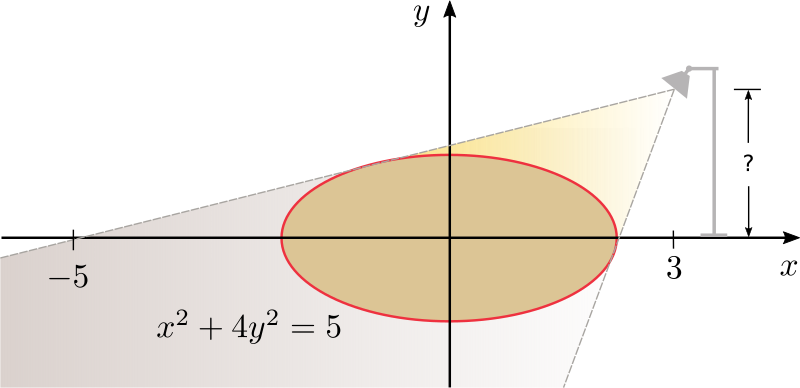
\includegraphics[width=8cm]{./png/3.5.67.png}
    \end{center}

\newpage

\item[3.6.49]
    Use logarithmic differentiation to find the derivative of the function $y = x^{x}$.

\vspace{6cm}

\item[3.6.62]
    Show that $\displaystyle \lim_{n \to \infty} \left( 1 + \frac{x}{n} \right)^{n} = e^{x}$ for any $x > 0$.

\vspace{6cm}

\item[3.6.82]
    \begin{enumerate}
        \item
            One way of defining $\sec^{-1}(x)$ is to say that $y = \sec^{-1}(x) \iff \sec (y) = x  $
            and $0 \leq  y < \frac{\pi }{2}$ or $ \pi \leq  y <  \frac{3\pi}{2}$.
            Show that, with this definition,
            \[
                \frac{d}{dx} \sec^{-1} (x) = \frac{1}{x \sqrt{x^{2} - 1}}.
            \]
        \item
            Another way of defining $\sec^{-1} (x) $ that is sometimes used it to say
            that $y = \sec^{-1} (x) \iff \sec (y) = x  $ and $0 \leq y \leq \pi $, $y \neq \frac{ \pi  }{2}$.
            Show that, with this definition,
            \[
                \frac{d}{dx} \sec^{-1} (x) = \frac{1}{|x| \sqrt{x^{2} - 1}}.
            \]
    \end{enumerate}

\newpage

\item[3.6.83]
    \textbf{Derivatives of Inverse Functions} Suppose that $f$ is a one-to-one differentiable
    function and its inverse function $f^{-1}$ is also differentiable. Use
    implicit differentiation to show that

    \[
        (f^{-1})'(x) = \frac{1}{f'(f^{-1}(x))}
    \]
    provided that the denominator is not $0$.

\vspace{6cm}

\item[3.6.85]
    Use the formula in \textbf{3.6.83}. If $f(x) = x + e^{x}$, find $(f^{-1})'(1)$.

\end{enumerate}
\end{document}
